\chapter{Diseño del prototipo}
    \section{Metodología}
        La metodología ágil \textit{Team Data Science Process} es adecuada para el prototipo a desarrollar, la cual provee los siguientes \textit{milestones} para desarrollar el modelo del agente conversacional:
        \begin{enumerate}
            \item Una fase enfocada al entendimiento del negocio. 
            \item Una fase enfocada a la adquisición de los recursos y el entendimiento de estos.
            \item Una fase enfocada al modelado empleando los datos obtenidos en la fase anterior.
            \item Una fase enfocada al despliegue en sus respectivos ambientes.
        \end{enumerate}
        
        \begin{description}
            \item[Entendimiento del negocio:] Esta fase se trata de identificar las variables clave para definir los objetivos del modelo. La correcta identificación de estas impactaran directamente en el éxito que pueda obtener el prototipo, tanto en su uso, viabilidad y desempeño. Para alcanzar este objetivo es indispensable:
                \begin{description}
                    \item [Definir objetivos:] Identificar las variables objetivo del modelo a implementar, basándose en las métricas para medir el grado de éxito ya sea por el área de oportunidad debido a la ausencia o mala implantación de una solución o por un análisis factible del negocio para así, desarrollar un plan de hitos los cuales se les asignará a miembros del equipo adjudicándoles ciertas responsabilidades.
                    \item [Identificar las fuentes de datos:] Pueden ser numerosas y variables. En el caso de este agente conversacional su principal fuente de datos serán las conversaciones de la página oficial de Facebook de la Escuela Superior de Cómputo {\bf ESCOM IPN MX}.
                \end{description}
            \item[Adquisición de recursos:] Habiendo identificando las fuentes de información contempladas en la fase de \textit{Entendimiento del negocio} y de acuerdo a la regla de negocio número cuatro, se obtendrán los recursos lingüísticos los cuales se les aplicara un proceso de transformación llamado ``normalización'' para obtener datos limpios y de calidad, dando lugar a un conjunto de datos relacionados con nuestras variables objetivo, estos datos serán almacenados y puestos a disposición para la siguiente fase.

            \item[Modelado:]
               Una vez obtenidos todos los recursos lingüísticos gracias a la fase de \textit{Adquisición de recursos}, se separara el conjunto en dos partes a los que llamaremos: ``conjunto de entrenamiento'' y ``conjunto de prueba'', con una distribución del conjunto original del 80\% y 20\% respectivamente, para construir el modelo con base en los datos de entrenamiento haciendo uso de algoritmos y técnicas de aprendizaje automático y procesamiento del lenguaje natural, para así evaluar el modelo resultante con los datos de prueba. 
               Si la precisión del modelo es suficiente se dará continuidad a la fase de \textit{Despliegue}, en caso contrario se identificará la fase cuyo resultado haya influenciado negativamente en el modelo resultante y se remontará a la fase en cuestión para realizar los cambios pertinentes.

            \item[Despliegue:]
                Se proveerá de una infraestructura para que nuestro modelo resultante pueda ser consumido por los servicios de \textit{Facebook}.
    
                
        \end{description}
        
    \section{Tecnologías}
        \begin{description}
            \item[Python:] Diseñado por Guido van Rossum en 1991, es un lenguaje de programación interpretado, dinámico y multiplataforma.
            Soporta programación orientación a objetos, programación imperativa y programación funcional.
            \item[NTKL:] Es un conjunto de bibliotecas y programas enfocadas al procesamiento del lenguaje natural.
            \item[GENSIM:] Es una biblioteca para el modelado de temas no supervisados y el procesamiento del lenguaje natural, que utiliza el aprendizaje automático moderno de estadística.
            \item[Docker:] Desarrollado por Solomon Hykes en marzo del 2013, es un software que ayuda a empaquetar aplicaciones dentro de un contenedor en el que se especifican las configuraciones y sus dependencias necesarias para que la aplicación embebida pueda correr, ofreciendo portabilidad, eficiencia, optimización de tiempo y recursos.
            
            \item[Docker compose:] Es un gestor de contenedores Docker con la característica de poder desplegar todo un entorno partir de un archivo YALM en el que se especifica paso por paso como conectar y configurar estos servicios.
            \item[MySQL:] Creada por David Axmark, Allan Larsson y Michael Widenius en 1995, es un gestor de bases de datos relacional.
            \item[MongoDB:] Desarrollado en el 2007 por la empresa \textit{10gen Inc}, es una base de datos distribuida de tipo NoSQL orientada a documentos en la cual se almacenan datos no estructurados en formato BSON.  
            \item[GitHub:] Creado en el 2010, es un repositorio de código que utiliza el sistema de control de versiones GIT.
            \item[Git:] Creado por  Linus Torvalds, es un software de control de versiones en el se lleva un registro de los cambios efectuados por los desarrolladores a los archivos de código fuente y así, llevar un mayor control en las versiones sobre las que se trabaja cada rama del proyecto.
            \item[\LaTeX:] Escrito por Leslie Lamport en 1984, está formado por un gran conjunto de macros de Tex el cual fue creado por Donald Knuth en 1978. Es un sistema de composición de textos, esta enfocado a la creación de documentos de gran calidad tipográfica.
            \item[Graph API:] es el núcleo de la pagina de Facebook y cuenta con las funciones de poder leer y escribir datos en Facebook, permite la conexión de aplicaciones externas que quieran consumir sus distintos servicios.
            \item[AWS:] plataforma cloud con servicios tipo \it{IaaS}, \it{PaaS} y \it{SaaS}.
        \end{description}
        
    \section{Modelado}
    El propósito de estos diagramas es para tener un mayor entendimiento de la funcionalidad y el comportamiento de nuestro sistema. A continuación de presentan los casos de uso, diagramas de procesos, diagramas de clases, el diagrama entidad-relación y finalmente los diagramas de infraestructura que conforman el de prototipo de agente conversacional.
    \subsection{Diagramas de casos de uso}
        Los diagramas de casos de uso sirven para especificar el comportamiento y comunicación del sistema mediante su interacción con los usuarios y otros sistemas. Nuestro agente conversacional a lo largo de su ciclo de vida tendrá interacción tanto con usuarios como con sistemas externos para lograr su perfecta ejecución. La figura \ref{fig:cu-scraper} describe como el usuario administrador ejecuta el micro servicio que lleva por nombre \textit{Scraper}, el cual se emplea como un modulo de extracción de mensajes, este se conecta con \textit{Graph API} gracias a un \textit{token} de acceso, permitiendo descargar los mensajes para después almacenarlos en el sistema local de archivos de la computadora o en una base de datos no relacional.
        \begin{figure}[H]
             \centering
             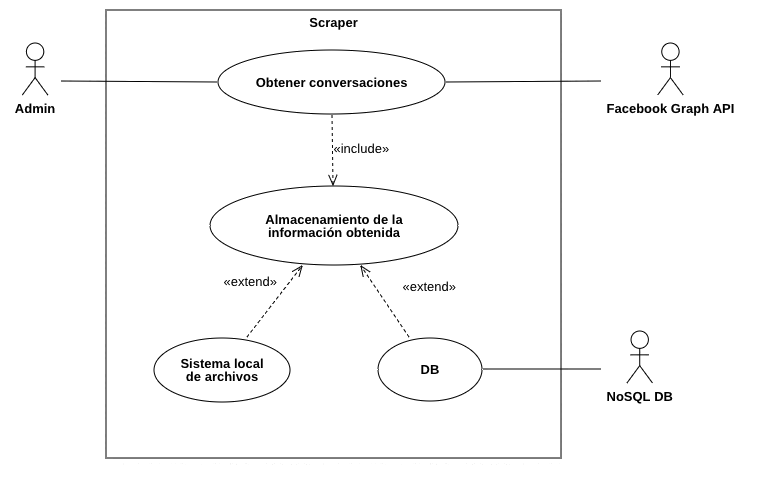
\includegraphics[height=10cm, width=16.5cm]{Latex/Classes/Imagenes/Scraper_cu.png}
             \caption{Diagrama de casos de uso para el modulo de extracción denominado \texit{Scraper}.}
             \label{fig:cu-scraper}
        \end{figure}
        La figura \ref{fig:cu-nlp-tp} describe una de las funcionalidades del modulo de procesamiento de lenguaje natural, en esta parte del proceso se trata de establecer una conexión con la base de datos no relacional donde los datos crudos obtenidos por \textit{Scraper} han sido almacenados, una vez que se han recuperados estos datos se realizada un paso denominado estandarización de texto, en el cual con ayuda de diccionarios de lemas y \textit{stopwords} se limpian los documentos dejando únicamente aquellas palabras relevantes, este proceso tiene muchas fases y cada una de estas son almacenadas en una base de datos relacional (véase la figura 4.7).
        \begin{figure}[H]
             \centering
             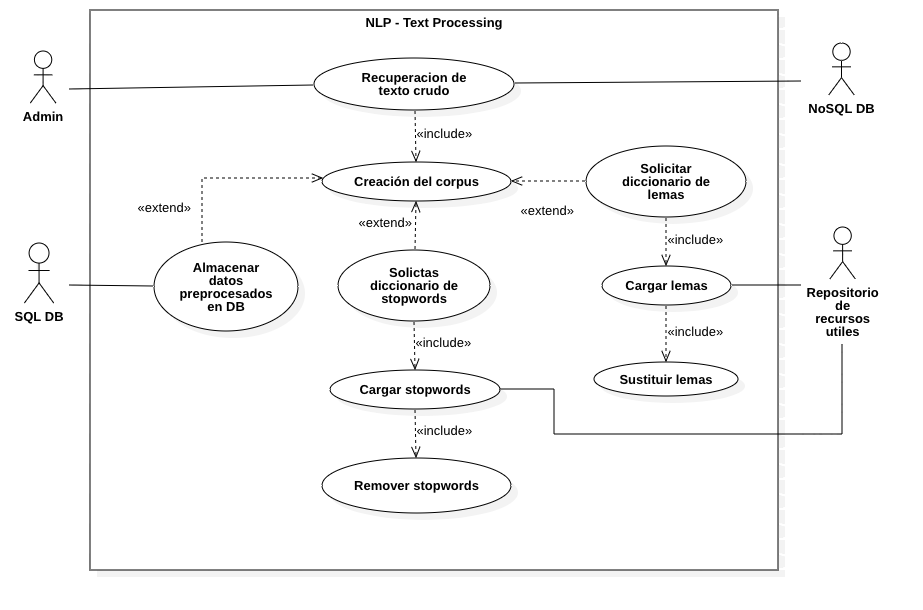
\includegraphics[height=14cm, width=16.5cm]{Latex/Classes/Imagenes/NLP_Text_Processing.png}
             \caption{Diagrama de casos de uso para el modulo de pre-procesamiento de texto.}
             \label{fig:cu-nlp-tp}
        \end{figure}
        La figura \ref{fig:cu-nlp-ta} describe otra de las funcionalidades del modulo de procesamiento de lenguaje natural, en el cual se obtienen los datos preprocesados de la base de datos relacional para aplicar el algoritmo \textbt{LDA} y poder extraer los temas frecuentes tratados dentro del texto.
        \begin{figure}[H]
             \centering
             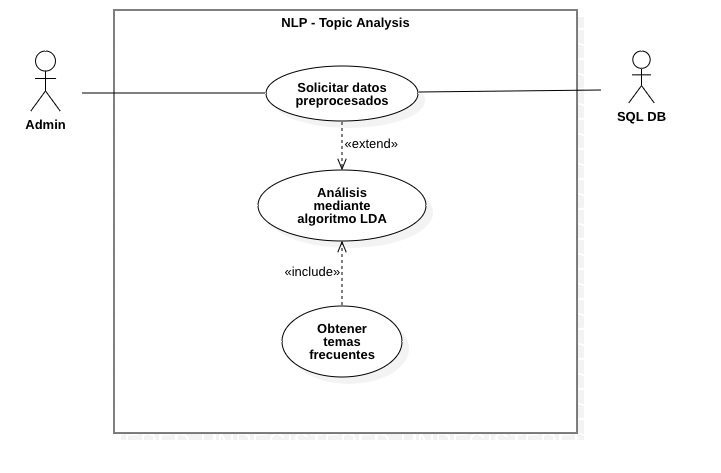
\includegraphics[height=8cm, width=16.5cm]{Latex/Classes/Imagenes/NLP_Topic_Analysis.png}
             \caption{Diagrama de casos de uso para el modulo de \textit{topic analysis}.}
             \label{fig:cu-nlp-ta}
        \end{figure}
        La figura \ref{fig:cu-nlp-g} describe la funcionalidad de graficación del modulo de procesamiento de lenguaje natural, el cual toma los datos que el algoritmo \textbf{LDA} arroja para graficarlos y que el usuario administrador pueda realizar un análisis visual de estos datos.
        \begin{figure}[H]
             \centering
             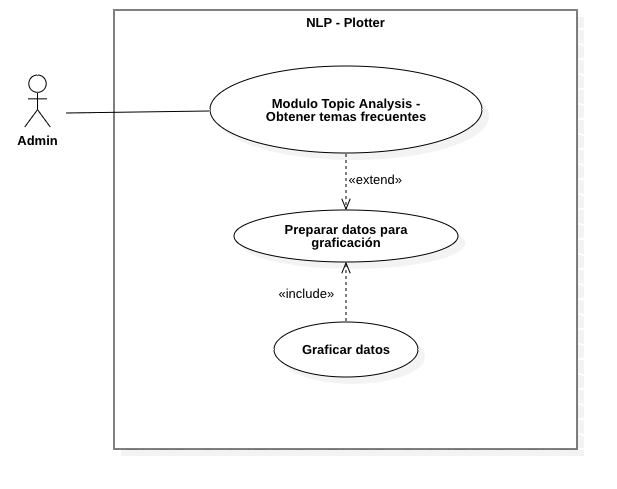
\includegraphics[height=8cm, width=16.5cm]{Latex/Classes/Imagenes/NLP_Plotter.png}
             \caption{Diagrama de casos de uso para el modulo de graficación.}
             \label{fig:cu-nlp-g}
        \end{figure}

    \subsection{Diagramas de procesos}
    Estos diagramas sirven para representar de manera gráfica un algoritmo o proceso. La figura \ref{fig:dp-scraper} muestra con mas detalle la funcionalidad del modulo \textit{Scraper} o de extracción. En primer lugar, este modulo espera recibir una serie de variables de entorno y banderas de entrada por parte del usuario, si la bandera de ``ayuda'' es percibida se muestra un mensaje de como usar el programa y se termina la ejecución, si no, entonces comienza el mapeo del resto de banderas, cabe destacar que estas banderas tienen un valor por defecto si el usuario no ingresa alguna. Una vez hecho esto entonces se busca por la bandera ``base de datos'', la cual si se encuentra en ``verdadero'' intentara establecer una conexión con la base de datos para almacenar ahí los mensajes, en dado caso de que la conexión no sea exitosa esta bandera automáticamente se cambia a ``flaso'' para prevenir futuros fallos y este registro se guarda en el sistema de \textit{logs}. Posteriormente se intenta establecer una conexión con \textit{Graph API}, si el \textit{token} es invalido se muestra un mensaje de error personalizado, se termina la ejecución y este error es almacenado en el sistema de \textit{logs}, en caso de una conexión exitosa comienza la descarga de mensajes, por cada mensaje se pregunta por la bandera de \textit{base de datos} para que, en caso de estar en ``verdadero'', el mensaje sea almacenado en la base de datos no relacional, de lo contrario el mensaje será almacenado en el sistema local de archivos. Una vez terminada la descarga de mensajes se termina la ejecución de este módulo. \break \break
    La figura \ref{fig:dp-nlp} muestra el flujo del módulo de procesamiento de lenguaje natural. En primer lugar, este modulo espera recibir una serie de variables de entorno y banderas de entrada por parte del usuario, si la bandera de ``ayuda'' percibida se muestra un mensaje de como usar el programa y se termina la ejecución, si no, entonces comienza el mapeo del resto de banderas, cabe destacar que estas banderas tienen un valor por defecto si el usuario no ingresa alguna. Posteriormente se intenta conectar con la base de datos relacional, en caso de una conexión fallida se muestra un mensaje de error personalizado, el registro se guarda en el sistema de \textit{logs} y se termina la ejecución, de lo contrario, busca que la bandera de \textit{pre-procesamiento} se encuentre en ``verdadero'', de ser así se intenta establecer una conexión con la base de datos no relacional, dándose el caso de una conexión fallida se muestra un mensaje de error personalizado, el registro se guarda en el sistema de \textit{logs} y se termina la ejecución, de lo contrario, se descargan los mensajes en su formato crudo para que por medio de diccionarios de lemas y \textit{stopwords} estos datos sean normalizados, cada uno de estos mensajes será guardado en la base de datos relacional. Luego, si la bandera de \textit{análisis LDA} se encuentra en ``verdadero'' y dada la columna de la base de datos relacional (véase la figura \ref{fig:diagrama-entidad-relacion}) especificada en las opciones de entrada, se procederá a descargar estos datos para realizar el análisis de tópicos, de lo contrario se finalizara la ejecución. Una vez realizado el análisis con el algoritmo \textbf{LDA} se pregunta si la bandera de \textif{graficación} esta en ``verdadero'', de ser así, entonces cada tópico propuesto por el algoritmo \textbf{LDA} sera graficado para realizar un análisis visual, en caso contrario los tópicos descubiertos serán almacenados en un archivo local para su futuro análisis, con este paso se terminal la ejecución del modulo de PLN.
        \begin{figure}[H]
             \centering
             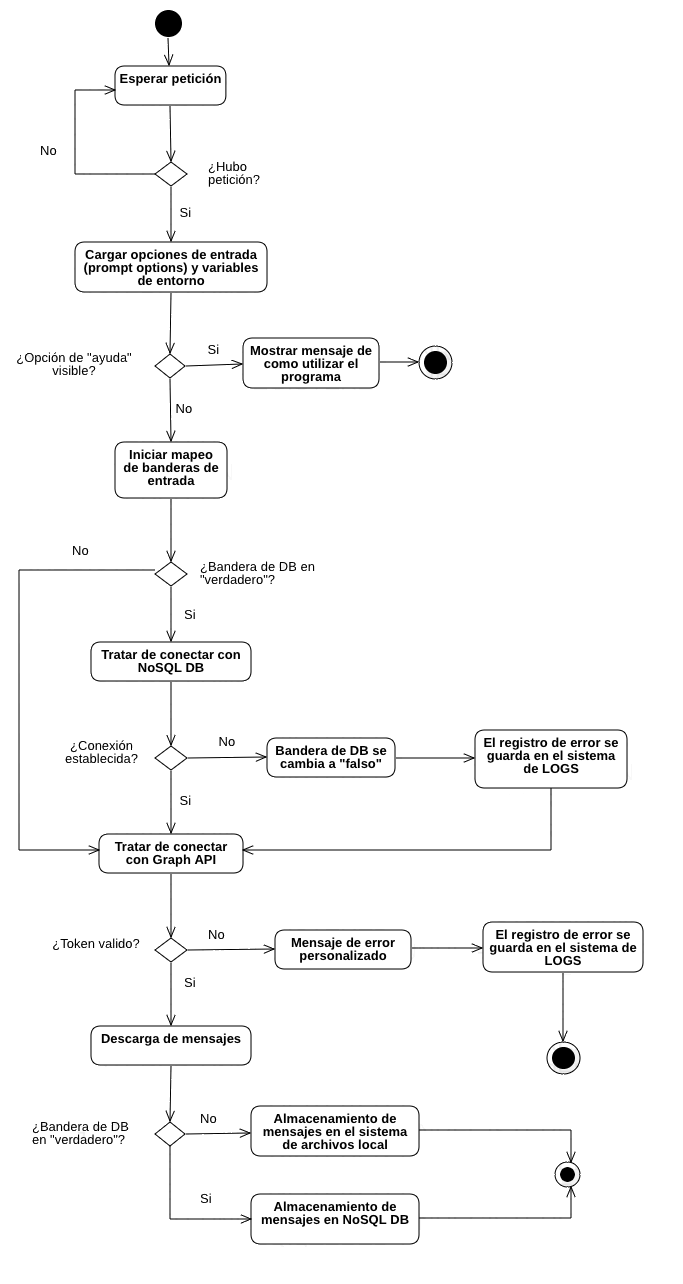
\includegraphics[height=18cm, width=16.5cm]{Latex/Classes/Imagenes/Scraper.png}
             \caption{Diagrama de procesos del módulo de extracción.}
             \label{fig:dp-scraper}
        \end{figure}
        \begin{figure}[H]
             \centering
             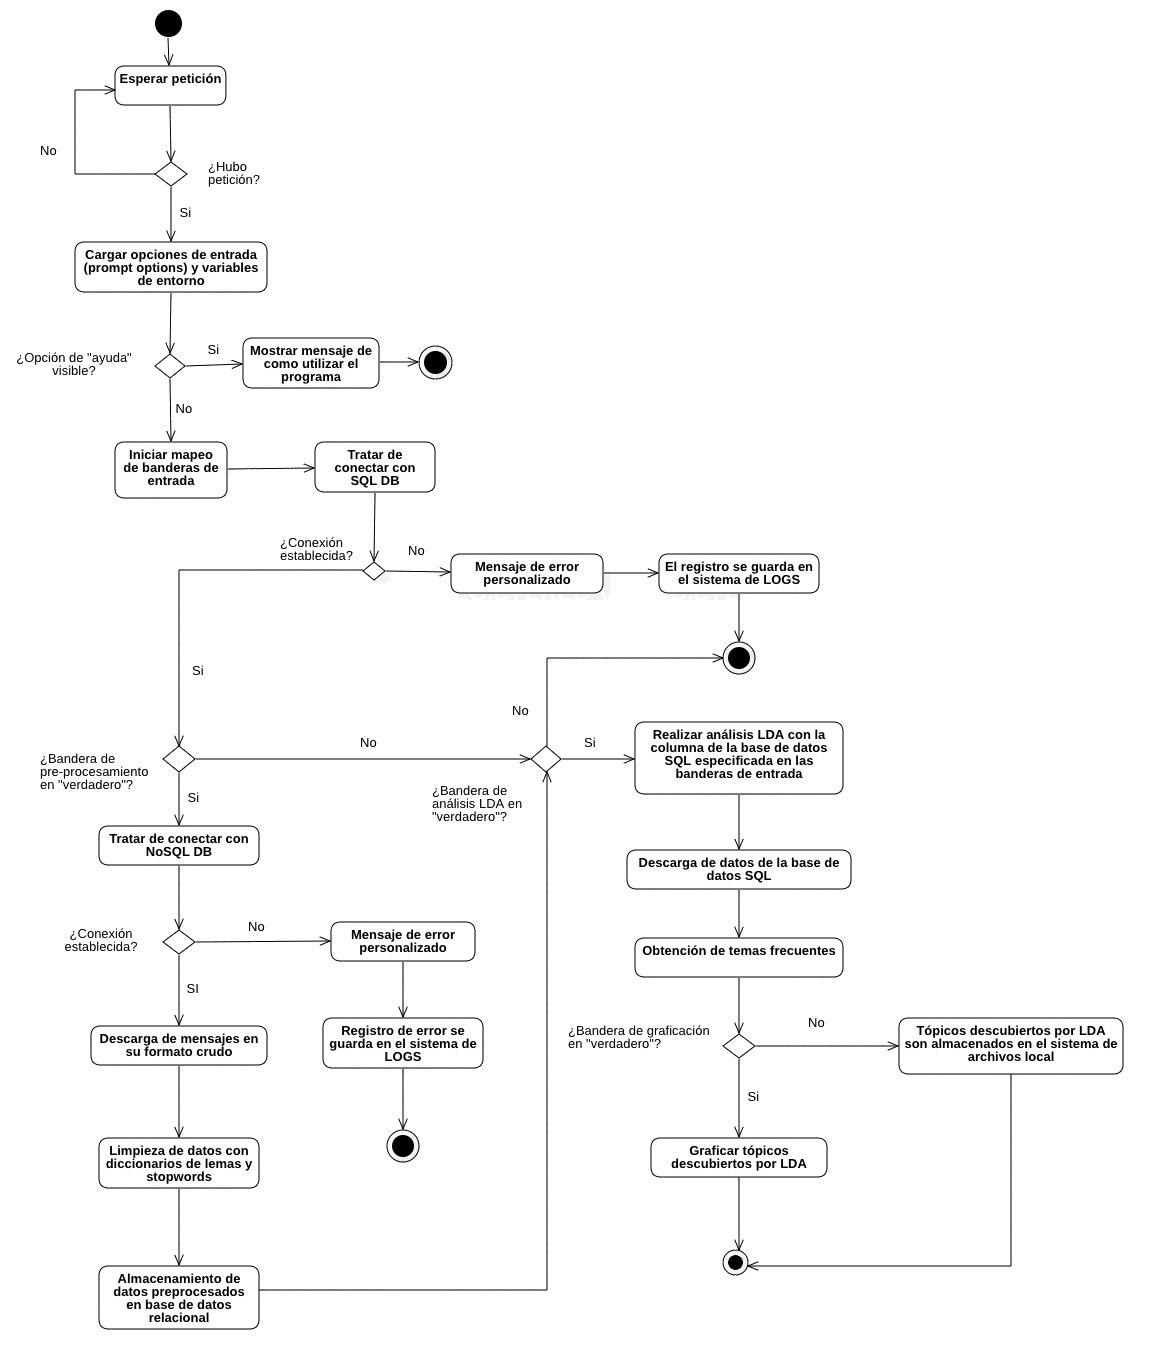
\includegraphics[height=20cm, width=16.5cm]{Latex/Classes/Imagenes/NLP.png}
             \caption{Diagrama de procesos del módulo de procesamiento de lenguaje natural.}
             \label{fig:dp-nlp}
        \end{figure}

    \subsection{Diagramas Entidad - Relación}
    El siguiente diagrama entidad-relación describe la base de datos relacional que será utilizada por el modulo de procesamiento de lenguaje natural, dicha base de datos cuenta únicamente con 2 tablas; \textit{Conversation}, que gurda una referencia de la conversación a la cual cada mensaje pertenece y \textit{Message} que almacena el mensaje en su formato crudo así como en distintos niveles de normalización.
    \begin{figure}[H]
         \centering
         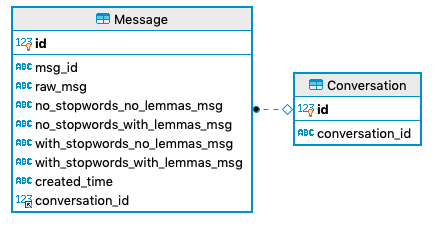
\includegraphics[width=.7\linewidth]{Latex/Classes/Imagenes/ER.png}
         \caption{Diagrama entidad-relación de la base de datos relacional.}
         \label{fig:diagrama-entidad-relacion}
    \end{figure}
    \newpage
        
    \subsection{Diagramas de clases}
        Los diagramas de clases mostrados en las figuras \ref{fig:dc-scraper} y \ref{fig:dc-nlp}, nos ayudan a entender de manera visual las clases que los módulos de \textit{extracción (scraper)} y \textit{procesamiento de lenguaje natural} utilizan, sus atributos, operaciones y las relaciones entre los objetos.
        \begin{figure}[H]
             \centering
             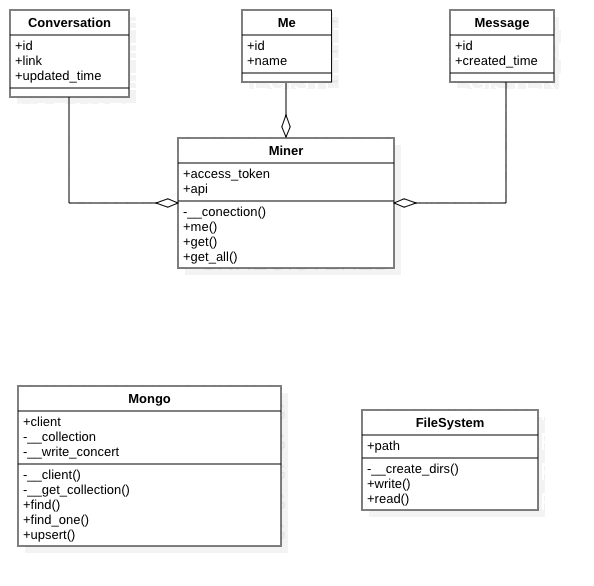
\includegraphics[height=9cm, width=16.5cm]{Latex/Classes/Imagenes/Scraper_Classes.png}
             \caption{Diagrama de clases del módulo \textit{Scraper} o de extracción.}
             \label{fig:dc-scraper}
        \end{figure}

        \begin{figure}[H]
             \centering
             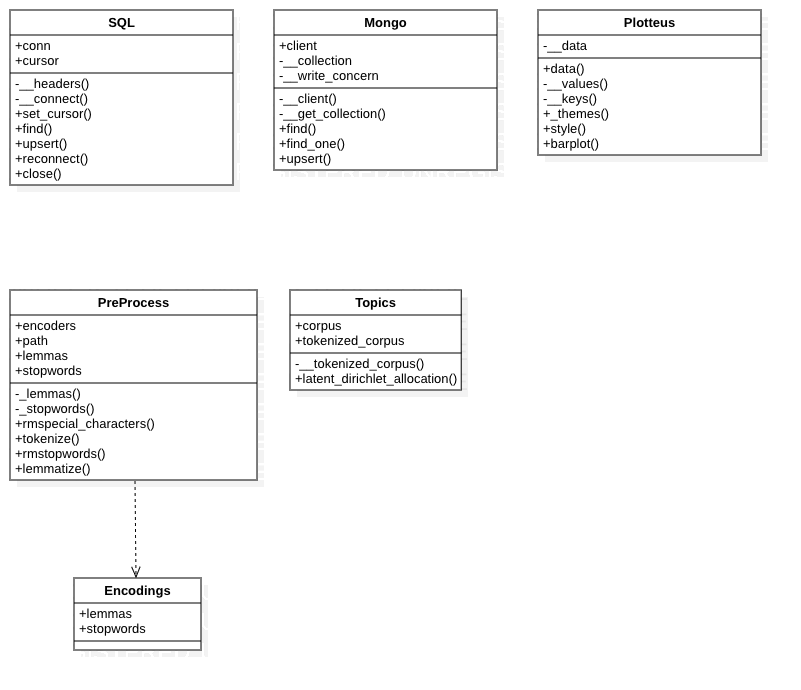
\includegraphics[height=9cm, width=16.5cm]{Latex/Classes/Imagenes/NLP_Classes.png}
             \caption{Diagrama de clases del módulo de procesamiento de lenguaje natural.}
             \label{fig:dc-nlp}
        \end{figure}
    \subsection{Diagramas de secuencia}
        El diagrama de secuencia de la figura \ref{fig:diagrama_secuencia} se muestra el proceso por el cual viaja una petición desde Facebook \textit{Graph API} hasta la infraestructura y como es tratado el dato:
        \begin{enumerate}
            \item La petición entra a una frontera \textit{AWS ACL} en el cual revisara que el no usuario se encuentre dentro de una black list
            \begin{enumerate}
                \item si esta: no permitirá el paso de trafico proveniente de ese usuario
                \item si no esta: redireccionará el trafico a \textit{API gateway}
                \begin{enumerate}

                    \item Llega a la frontera \textit{API gateway} el cual encolara la función control \textit{AWS Lambda} "StateMachine" dentro de la entidad \textit{AWS SQS}
                    \item La entidad \textit{AWS SQS} desencolara las anteriores peticiones de funciones control \textit{AWS Lambda} una por una de manera cronológica, "StateMachine" será desplegado al llegar al principio del encolador.
                    \item La función control \textit{AWS Lambda} "StateMachine" encolara dentro de una entidad \textit{AWS SQS} la función correspondiente al estado de la pregunta.
                    \begin{enumerate}
                        \item si el usuario es nuevo o nueva pregunta: la función a encolar será "Welcome"
                        \begin{enumerate}
                            \item La entidad \textit{AWS SQS} siguiendo el mismo principio del punto 3 invocará la funcion control \textit{AWS Lambda} "Welcome"
                            \item si el mensaje contenía una pregunta, se analizará y guardará el contexto dentro de la entidad \textit{AWS Elasticache}
                            \item La entidad \textit{AWS Elasticache} devolverá el estado de la petición a la funcion control \textit{AWS Lambda} "Welcome" tras haber guardado el contexto
                            \item La funcion control \textit{AWS Lambda} "Welcome" enviará la respuesta a la frontera \textit{API gateway}
                        \end{enumerate}
                        \item si es sobre preguntas pasadas: la función a encolar será "FAQs"
                        \begin{enumerate}
                            \item La entidad \textit{AWS SQS} siguiendo el mismo principio del punto 3 invocará la funcion control \textit{AWS Lambda} "FAQs"
                            \item La funcion control \textit{AWS Lambda} "FAQs" solicitará a la entidad \textit{AWS Elasticache} el contexto
                            \item La entidad \textit{AWS Elasticache} devolverá el contexto a la función control \textit{AWS Lambda} "FAQs"
                            \item La funcion control \textit{AWS Lambda} "FAQs" tras analizar la pregunta guardara el contexto dentro de la entidad \textit{AWS Elasticache}
                            \item si el mensaje contenía una pregunta, se analizará y guardará el contexto dentro de la entidad \textit{AWS Elasticache}
                            \item La entidad \textit{AWS Elasticache} devolverá el estado de la petición a la funcion control \textit{AWS Lambda} "FAQs" tras haber guardado el contexto
                            \item La funcion control \textit{AWS Lambda} "FAQs" enviará la respuesta a la frontera \textit{API gateway}
                        \end{enumerate}
                    \end{enumerate}
                    \item La frontera \textit{API gateway} actualizara las ACL de la frontera \textit{AWS ACL}
                    \item La frontera \textit{API ACL} se comunicará con Facebook \textit{Graph API} y retornara el resultado del análisis.
                    \item El paso 1.a.1 se repite hasta que la función control \textit{AWS Lambda} "StateMachine" pasa al estado "Fairwell"
                    \item La petición entra a una frontera \textit{AWS ACL} siguiendo la logica del paso 1
                    \item Llega a la frontera \textit{API gateway} el cual encolara la función control \textit{AWS Lambda} "StateMachine" dentro de la entidad \textit{AWS SQS}
                    \item La entidad \textit{AWS SQS} siguiendo el mismo principio del punto 3 invocará la funcion control \textit{AWS Lambda} "StateMachine"
                    \item La función control \textit{AWS Lambda} "StateMachine" encolara dentro de una entidad \textit{AWS SQS} la función "Fairwell"
                    \item Llega a la frontera \textit{API gateway} el cual encolara la función control \textit{AWS Lambda} "Fairwell" dentro de la entidad \textit{AWS SQS}
                     \item La funcion control \textit{AWS Lambda} "Fairwell" enviará la respuesta a la frontera \textit{API gateway}
                     \item La frontera \textit{API gateway} actualizara las ACL de la frontera \textit{AWS ACL}
                    \item La frontera \textit{API ACL} se comunicará con Facebook \textit{Graph API} y retornara la respuesta
                \end{enumerate}
            \end{enumerate}


            
            \item La entidad \textit{AWS SQS} desencolara los mensajes de forma ordenada lanzando otra función control \textit{AWS Lambda} para cada una de estas.
            \item La función control \textit{AWS Lambda} analizara la petición y buscará en la entidad \textit{AWS Elacticache} un contexto de preguntas pasadas.
            \item La entidad \textit{AWS Elasticache} buscara si existe un contexto previo, si existe entonces retornará este, en caso contrario solo mandará una notificación.
            \item La función control \textit{AWS Lambda} analizara el mensaje obtenido con base en el resultado de la entidad \textit{AWS Elacticache}  y devolverá el resultado a la frontera \textit{API gateway}.
            \item La frontera \textit{API gateway} se comunicará con Facebook \textit{Graph API} y retornara el resultado del análisis.
        \end{enumerate}
        
        \begin{figure}[H]
             \centering
             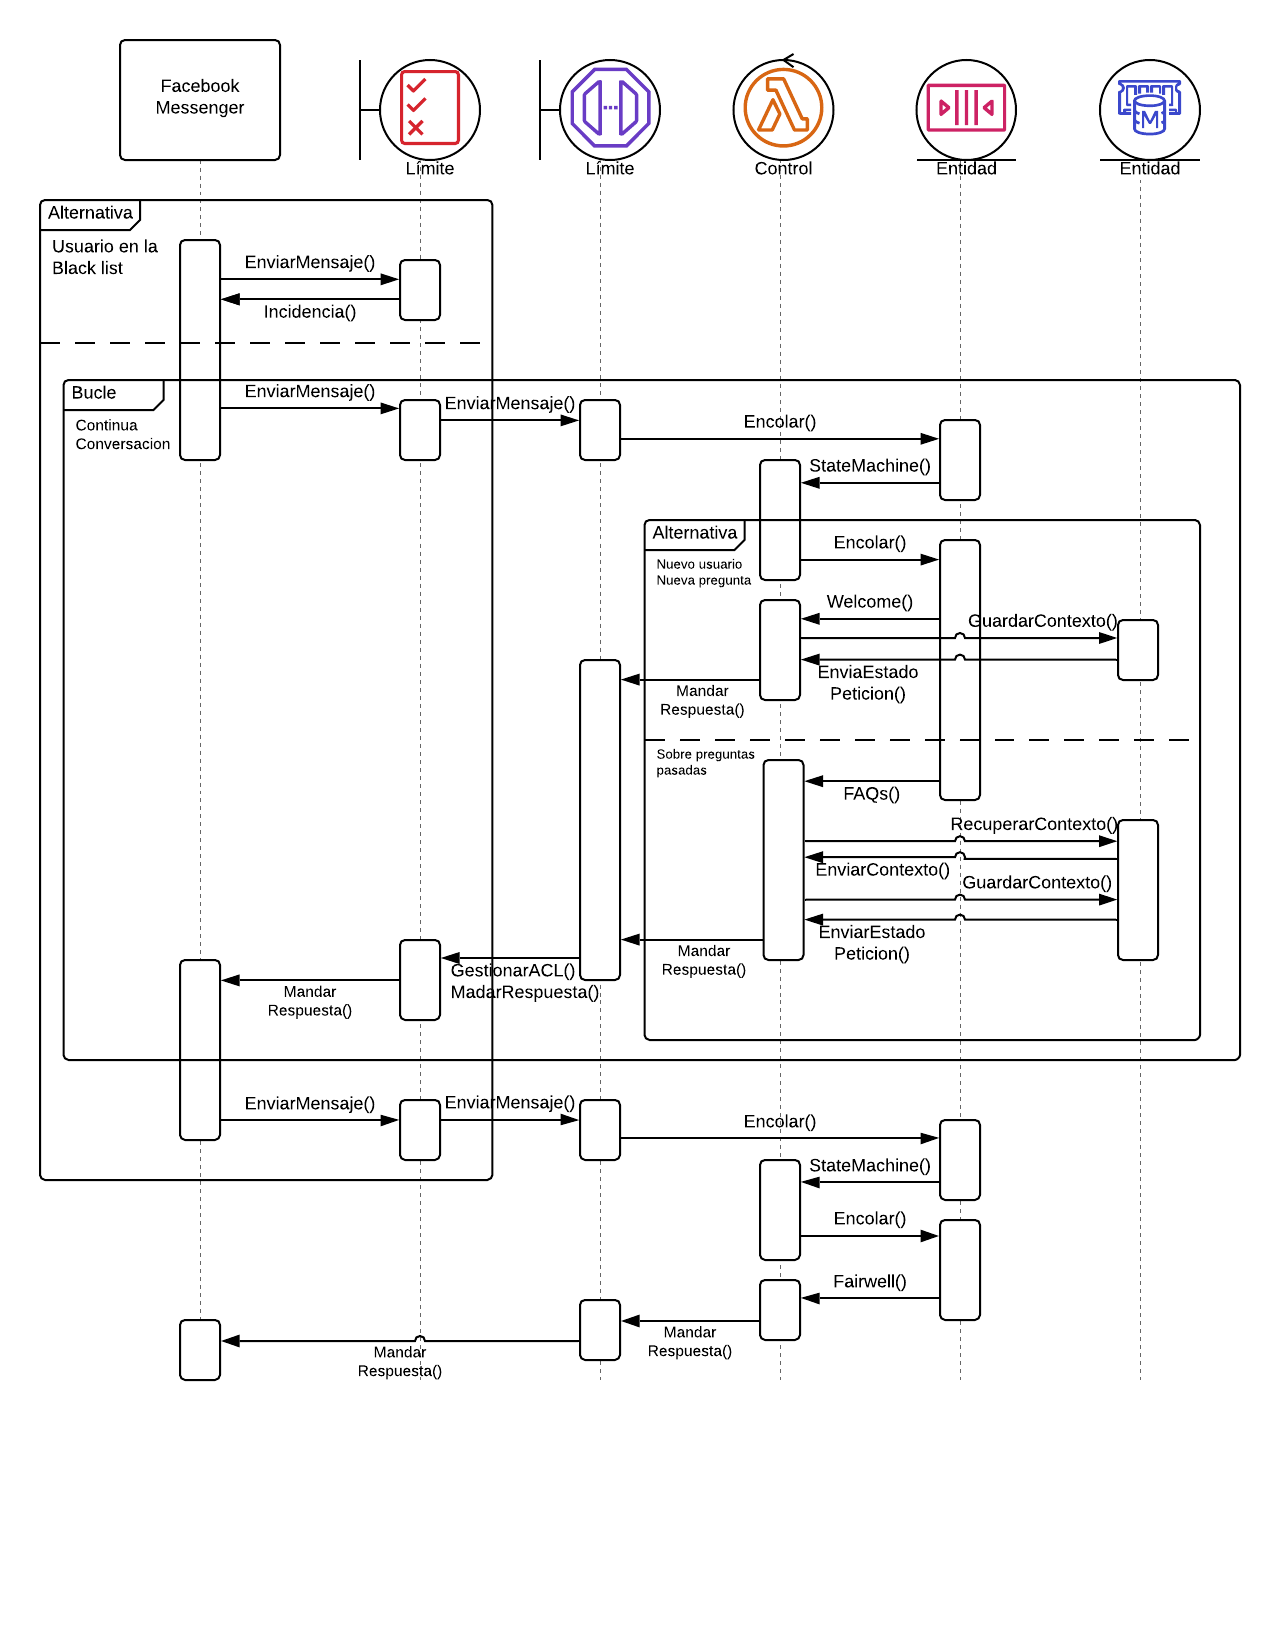
\includegraphics[height=14cm, width=16.5cm]{Latex/Classes/Imagenes/Diagrama_de_secuencia_del_sistema.png}
             \caption{Secuencia por la que viaja una pregunta dentro de las tecnologías de \textit{AWS}.}
             \label{fig:diagrama_secuencia}

        \end{figure}
    
    \subsection{Diagramas de infraestructura}
    
        El diagrama de infraestructura de la figura ~\ref{fig:infraestructura} se muestra la infraestructura sobre la cual se ejecutará el prototipo de agente conversacional, la implementación de este sera sobre el proveedor de computo en la nube \textit{AWS}.
        
        \textit{AWS Route 53} proveerá de los certificados necesarios para poder comunicar la tecnología \textit{AWS API Gateway} con Facebook \textit{Graph API} por medio de un canal bidireccional con las funciones de \textit{AWS Lambda} para mandar y recibir peticiones. \textit{AWS Lambda} ejecutará bloques de código cuando sea invocado retornando un resultado, \textit{AWS SQS} proveerá un sistema de encolamiento de mensajes de las peticiones entrantes y se definirá la acción de invocar una función de \textit{AWS Lambda} a la hora de desencolar estos. \textit{AWS Elasticache} proveerá una memoria temporal definida por el administrador, en el que se almacenan objetos de alta transaccionalidad de tipo clave valor. En el ambiente de despliegue, si se realiza un cambio sobre el código de una función de \textit{AWS Lambda} está se actualizará y se desplegara de tal manera que las nuevas funciones de \textit{AWS Lambda} corran con estos cambios.
        \begin{figure}[H]
             \centering
             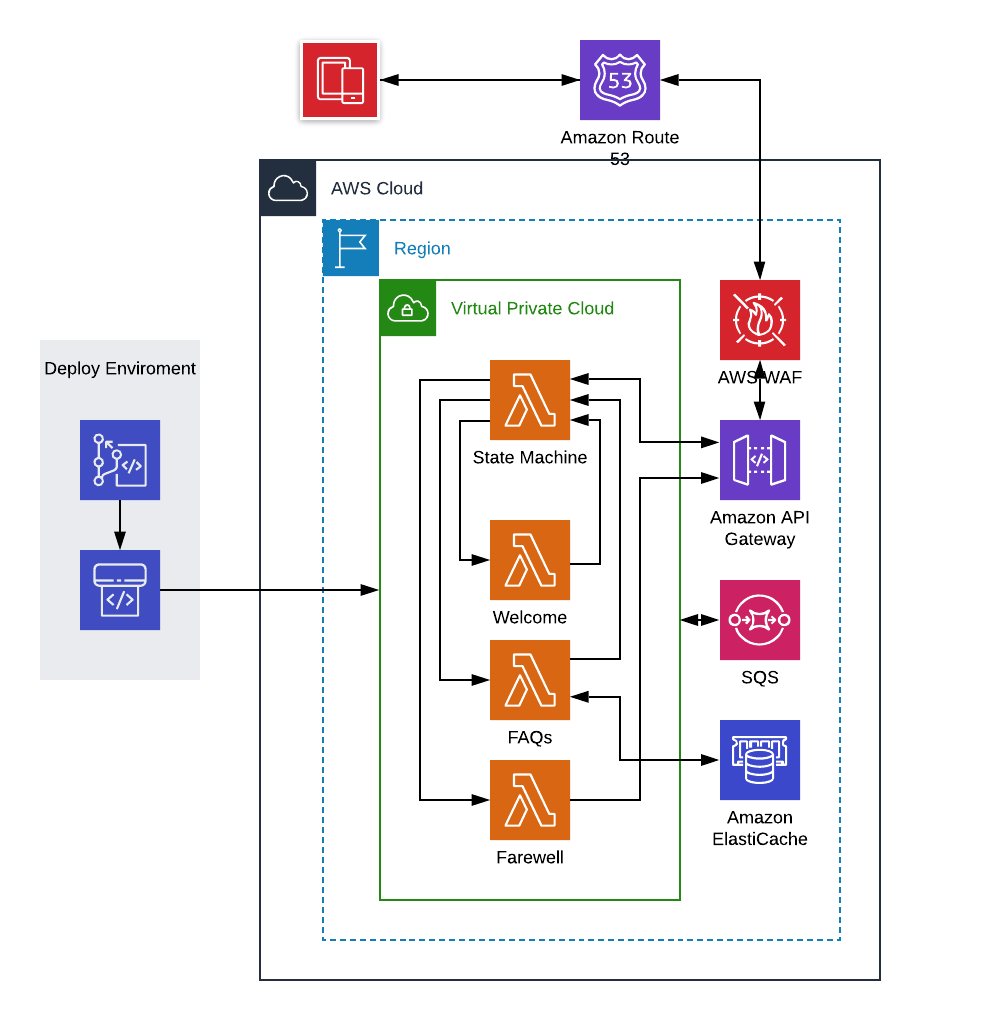
\includegraphics[height=12cm, width=16.5cm]{Latex/Classes/Imagenes/Diagrama_de_infraestructura.png}
             \caption{Infraestructura del agente conversacional}
             \label{fig:infraestructura}
        \end{figure}
        
        El diagrama de infraestructura de la figura  ~\ref{fig:infraestructuraExtraccionNLP} muestra dos módulos del prototipo de agente conversacional: Extracción y procesamiento de lenguaje natural.
        En el modulo de extracción se hace uso de un equipo de cómputo con salida a internet, se comunicará con \textit{Graph API} y obtendrá los datos pertinentes, sobre este equipo se ejecutará un contenedor de Docker con persistencia en el que correrá una base de datos NoSQL en una subnet privada con comunicación de tipo puente con el equipo de cómputo y se almacenarán los datos obtenidos.
        En el modulo de NLP, se hace uso de un equipo de cómputo en el que se ejecutarán dos contenedores con persistencia en una subnet privada con comunicación de tipo puente con el equipo de cómputo, los datos almacenados en la base de datos NoSQL pasaran por un submodulo de preprocesado y serán almacenados en la base de datos SQL. Con base a estos datos se ejecutará el submodulo de análisis de tópicos, al finalizar se comunicara internamente con el equipo y este ejecutará el submodulo de graficación.
        \begin{figure}[H]
             \centering
             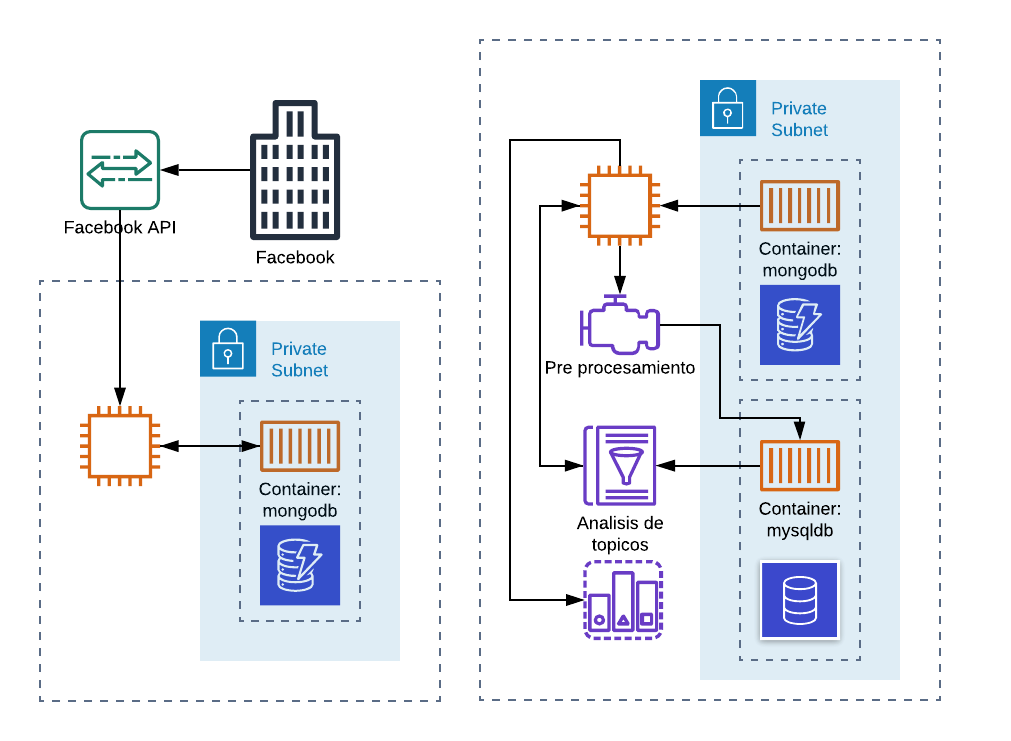
\includegraphics[height=12cm, width=16.5cm]{Latex/Classes/Imagenes/Diagramas_de_modulos.png}
             \caption{Infraestructura de los modulo de extracción y NLP respectivamente}
              \label{fig:infraestructuraExtraccionNLP}

        \end{figure}
    \subsection{Construcción del modelo}
    
        Es importante remarcar el hecho de que nuestro agente conversacional estará basado en un dominio de espacio cerrado enfocado a la resolución de preguntas frecuentes correspondientes al área de administración educativa, las respuestas obtenidas por este, estarán basadas en un modelo generativo.
        Se plantea el uso de mecanismos de atención el cual se encargará de dirigir la conversación hacia una pregunta especifica.
        
        La arquitectura interna del modelo esta basada en \it{Seg2Seg} el cual cuenta con tres capas de redes neuronales recurrentes con diferentes conjuntos de parámetros, una capa se encargará de codificar la secuencia de la fuente y la otra en decodificar la secuencia codificada por la anterior red neuronal 
        
        \begin{description}
        \item [Codificador:] Se encarga de obtener los datos de la pregunta y se entrenará con ellos, pasando la información a cada una se sus neuronas por medio de una cinta de memoria, al llegar al final, se mandará el estado junto con una cadena de inicio a la siguiente red neuronal, a partir de estos datos se generaran las respuestas.
        \end{description}
        \begin{figure}[H]
             \centering
             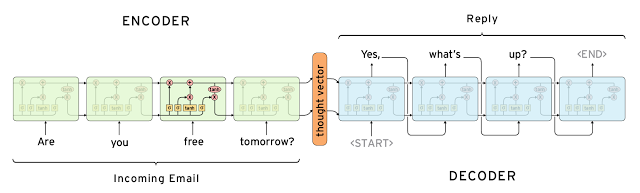
\includegraphics[height=7cm, width=16.5cm]{Latex/Classes/Imagenes/seg2seg.png}
             \caption{Arquitectura \it{Seg2Seg}}
              \label{fig:infraestructuraExtraccionNLP}
        \end{figure}
        
        Las redes neuronales dentro de estas dos capas son del tipo \it{LSTM} los cuales son una variante de las \it{RRN}, cuentan con una célula de memoria el cual esta compuesta por 3 principales compuertas:
        
        
        \begin{description}
            \item [Forget gate:] se encarga de analizar la entrada junto al estado de la \it{LSTM}, y pasar estos por medio de una fusión de activación de tipo \it{sigmoidal}, se eliminaran los datos que no serán usados en adelante.
            \item [Output gate:] después de aplicar las transformaciones de la cinta con la salida de la \it{Forget gate} y transformando esta con el resultado de \it{Update gate}, transformaremos el resultado con una función \it{Tanh} a la cinta de memoria y la pasaremos por una compuerta \bf{XOR} con la entrada junto al estado de la \bf{LSTM}, ya pasados por la fusión de activación de tipo \it{sigmoidal}, generaremos así la salida del nuevo estado.
        \end{description}
        
          \begin{figure}[H]
             \centering
             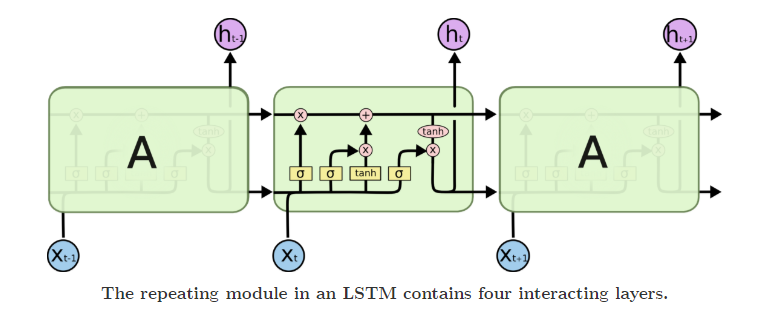
\includegraphics[height=7cm, width=16.5cm]{Latex/Classes/Imagenes/LSTM.png}
             \caption{Arquitectura de la LSTM}
              \label{fig:infraestructuraExtraccionNLP}
        \end{figure}
        
        La tercera capa es un mecanismo de atención, enfocado en generar respuestas recomendadas con base al contexto de los estados de cada neurona del codificador junto a la intención obtenida por el modulo de \it{LDA}. 
        \begin{figure}[H]
             \centering
             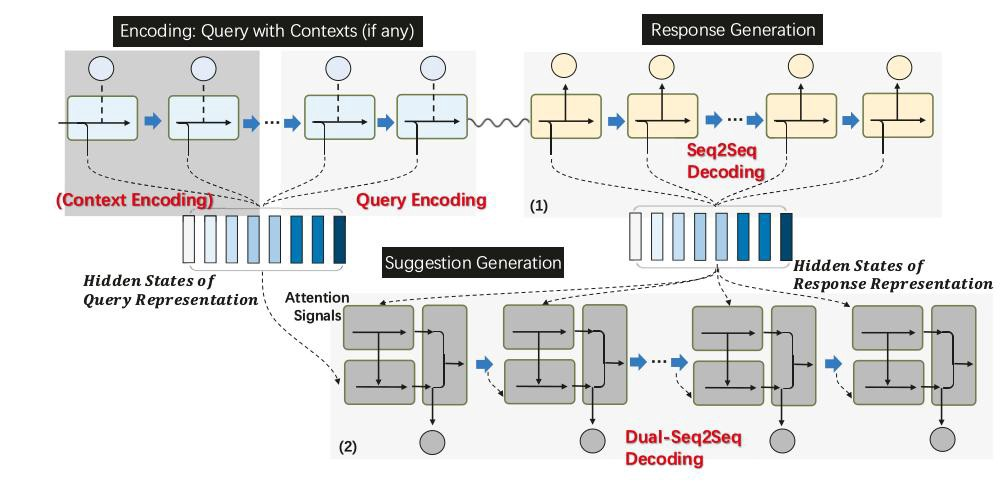
\includegraphics[height=12cm, width=16.5cm]{Latex/Classes/Imagenes/attention.jpeg}
             \caption{Arquitectura del mecanismo de atención}
              \label{fig:infraestructuraExtraccionNLP}
        \end{figure}
    \subsection{Resultados esperados}
        \begin{figure}[H]
             \centering
             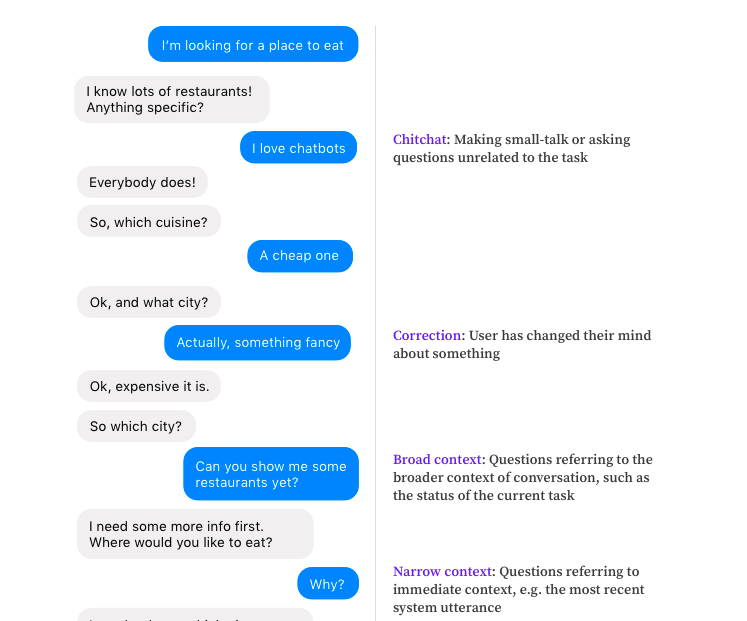
\includegraphics[height=12cm, width=16.5cm]{Latex/Classes/Imagenes/hola.png}
             \caption{Resultados esperados usando la técnica de \it{Seg2Seg} con mecanismos de atención}
              \label{fig:infraestructuraExtraccionNLP}
        \end{figure}
        
    Cabe destacar que este modelo estará delimitado por una cierta cantidad de preguntas a resolver, como ya se menciono, será un sistema cerrado enfocándose principalmente en 3 tipos de peticiones:
    
    \begin{itemize}
        \item Convocatorias de inscripción, tanto semestrales como Trabajos Terminales, protocolo de TT, electiva, optativa y postgrados.
        \item Información para la baja de unidades de aprendizaje así como baja temporal o definitiva.
        \item Información general para alumnos de nuevo ingreso sobre la Escuela Superior de Cómputo.
    \end{itemize}